% (c) 2015 Daniele Zambelli daniele.zambelli@gmail.com

% \section{TODO}

\section{Esercizi}

\subsection{Esercizi dei singoli paragrafi}

\subsubsection*{\numnameref{sec:ellisse_}}


% \begin{esercizio}
% \label{ese:D.19}
% testo esercizio
% \end{esercizio}
% 
% \begin{esercizio}\label{ese:03.1}
% Consegna:
%  \begin{enumeratea}
%   \item  
%  \end{enumeratea}
% \end{esercizio}

L'ellisse come luogo geometrico
\begin{esercizio}
  \label{ese:div.003}
  Per ciascuna delle seguenti ellissi determina il semiasse a, il 
semiasse b e le coordinate dei fuochi, infine scrivine l'equazione.
\begin{figure}[htbp]
  \centering%
  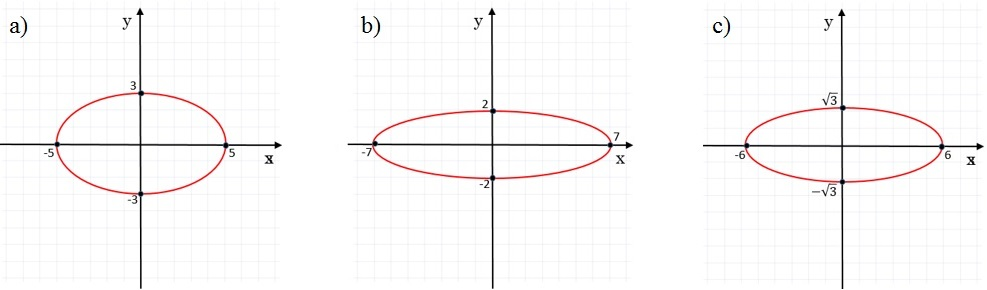
\includegraphics[height=16cm, width=12cm, keepaspectratio] {img/ellissi3.jpg}%
  %\caption{Generazione di un cono a due falde}%
\end{figure}
\end{esercizio}
Le caratteristiche dell'ellisse\\

\begin{esercizio}
  \label{ese:div.003}
  Determina i semiassi a e b ed i fuochi delle seguenti ellissi.
  \begin{enumeratea}
    \item $\dfrac{x^{2}}{16} + \dfrac{y^{2}}{9} =1$ 
    \hfill
      $\left[a=4; b=3;~F_{1} \left( 
\sqrt{7};~0\right),~F_{2}~\left(- \sqrt{7};~0\right)\right]$
    \item $ \dfrac{x^{2}}{49} + \dfrac{y^{2}}{25} =1$  
    \hfill
      $\left[a=7; b=5;~F_{1}~\left(2 
\sqrt{6};~0\right),~F_{2}~\left(-2 \sqrt{6};~0\right)\right]$
      \item $ \dfrac{x^{2}}{20} + \dfrac{y^{2}}{14} =1$
      \hfill $\left[a=2 \sqrt{5} ;~ b= \sqrt{14} ;  F_{1}  
\left(\sqrt{6} ;~ 0\right),  F_{2}  \left(-\sqrt{6} ;~0\right)\right]$
      \item $ \dfrac{x^{2}}{169} + \dfrac{y^{2}}{81} =1$
      \hfill $\left[a=13 ;~b=11 ;~F_{1}  \left(4 \sqrt{3} 
;~0\right),~F_{2}  \left(-4 \sqrt{3} ;~0\right)\right]$
      \item $ \dfrac{x^{2}}{36} + \dfrac{y^{2}}{8} =1$
      \hfill $\left[a=6 ;~b=2 \sqrt{3}  ;~F_{1}  \left(2 \sqrt{7} 
;~0\right),  F_{2}  \left(-2 \sqrt{7} ;~0\right)\right]$
      
      \item  $4 {x^{2}} +{y^{2}} =32$
      \hfill $\left[a=2 \sqrt{2}  ;~b=2 ;  ~F_{1}  (2;~0), ~ F_{2}  
(-2;~ 0)\right]$
  \end{enumeratea}
\end{esercizio}

% \subsubsection*{12.2 - Polinomi in più variabili}
% 
\begin{esercizio}
  \label{ese:div.003}
  Per ciascuna delle seguenti ellissi determina i quattro vertici, la 
semidistanza focale c e l'eccentricità, infine disegnala nel piano 
cartesiano.
  \begin{enumeratea}
\item $ \dfrac{x^{2}}{9} + \dfrac{y^{2}}{5} =1$  
\hfill $\left[A(\pm3;~0), B\left(0; ~ \pm  \sqrt{5} \right); ~c=2 ;~ e= 
\dfrac{2}{3} \right]$
\item $ \dfrac{x^{2}}{144} + \dfrac{y^{2}}{64} =1$  
\hfill $\left[A(\pm12;~ 0), B(0; ~ \pm ); ~c=4 \sqrt{5}  ;~ e= 
\dfrac{\sqrt{5}}{3} \right]$

\item $ \dfrac{x^{2}}{196} + \dfrac{y^{2}}{4} =1$
\hfill $\left[A(\pm14;~ 0),~ B(0; ~ \pm 2);~ c=8 \sqrt{3}  ;~ e= 
\dfrac{4\sqrt{3}}{7} \right]$

\item $8{x^{2}}+9{y^{2}}=72$
\hfill  $\left[A(\pm3; 0),~ B\left(0;~ \pm 2 \sqrt{2} \right);~c=1; ~e= 
\dfrac{1}{3} \right]$

\item ${x^{2}}+7{y^{2}}=49$
\hfill $\left[A(\pm7; 0),~ B\left(0; ~ \pm  \sqrt{7} \right);~ c= \sqrt{42} 
;~ e= \sqrt{\dfrac{6}{7}} \right]$

\item $ \dfrac{x^{2}}{16} + y^{2} =1$  
\hfill $\left[A(\pm4; 0),~ B(0;  \pm 1);~ c= \sqrt{15}  ;~ e= 
\dfrac{\sqrt{15}}{4} \right]$

  \end{enumeratea}
\end{esercizio}
L'ellisse con fuochi appartenenti all'asse Y
\begin{esercizio}
  \label{ese:div.003}
   Tra le seguenti ellissi riconosci quelle aventi i fuochi sull'asse 
Y e disegnale. \\
a) $ \dfrac{x^{2}}{16} + y^{2} =1$  \hspace{1.5cm} b) $ \dfrac{x^{2}}{4} + 
\dfrac{y^{2}}{16} =1$\hspace{1.5cm}  c) $ \dfrac{x^{2}}{9} + 
\dfrac{y^{2}}{36} =1$\hspace{1.45cm} d) $2 x^{2} +4y^{2} =16$\\
e) $16 x^{2} +9 y^{2} =144$  \hspace{0.7cm} f) $ \dfrac{x^{2}}{25} + 
\dfrac{y^{2}}{49} =1$\hspace{1.6cm}  g) $9 x^{2} +25 y^{2} =225$ 
\hspace{0.6cm} h) $ \dfrac{x^{2}}{2} + \dfrac{y^{2}}{9} =1$ 
\end{esercizio}
Condizioni per determinare l'equazione dell'ellisse
\begin{esercizio}
  \label{ese:div.003}
  Determina l'equazione dell'ellisse conoscendo i due elementi 
specificati, potendo essi essere a, b, e, un fuoco $ F_{1}$, i punti 
dell'ellisse $ P_{1} $ e $ P_{2} $ oppure i vertici $ A_{1} $, $ B_{1} $.
  \begin{enumeratea}
   \item a=12,\quad b=7
   \hfill $\left[ \dfrac{x^{2}}{144} + \dfrac{y^{2}}{49} =1\right]$
   \item a=6,\quad b=$ \dfrac{2}{3} $
   \hfill $\left[ \dfrac{x^{2}}{36} + \dfrac{9y^{2}}{4} =1\right]$
   \item e=$ \dfrac{3}{5} $,\quad $ F_{1}$(3; 0)
   \hfill $\left[ \dfrac{x^{2}}{25} + \dfrac{y^{2}}{16} =1\right]$
   \item e=$ \dfrac{2}{3} $,\quad $ F_{1}$(4; 0)
   \hfill $\left[ \dfrac{x^{2}}{36} + \dfrac{y^{2}}{20} =1\right]$
   \item $ P_{1}  \left(2; ~ \dfrac{2\sqrt{5}}{3} \right),~  P_{2} \left( 
\dfrac{3\sqrt{3}}{2}; ~ 1\right)$
   \hfill $\left[ \dfrac{x^{2}}{9} + \dfrac{y^{2}}{4} =1\right]$
   \item $ P_{1} \left( \dfrac{5}{3} ; ~ \dfrac{2}{3} \right), ~  P_{2} 
\left( \sqrt{2} ; ~ \sqrt{\dfrac{3}{5}} \right)$
   \hfill $\left[ \dfrac{x^{2}}{5} + y^{2} =1\right]$
   \item $ F_{1}\left( \sqrt{15} ;~ 0\right),~ A_{1}\left(2 \sqrt{5} ;~ 
0\right)$
   \hfill $\left[\dfrac{x^{2}}{20} + \dfrac{y^{2}}{5} =1\right]$
   \item $ F_{1}(6; 0),~ A_{1}\left(2 \sqrt{10} ; ~0\right)$
   \hfill $\left[ \dfrac{x^{2}}{40} + \dfrac{y^{2}}{4} =1\right]$
   \item  $e= \dfrac{3}{4} ,~ P_{1}\left(3; ~ \dfrac{7}{4} \right)$
   \hfill  $\left[ \dfrac{x^{2}}{16} + \dfrac{y^{2}}{7} =1\right]$
   \item $e= \dfrac{1}{2} ,~ P_{1}\left( \sqrt{\dfrac{8}{3}} ;~ 1\right)$
   \hfill $\left[ \dfrac{x^{2}}{4} + \dfrac{y^{2}}{3} =1\right]$
  
  \end{enumeratea}
\end{esercizio}

% \subsection{Esercizi riepilogativi} TODO
% 
% \begin{esercizio}
% \label{ese:D.19}
% testo esercizio
% \end{esercizio}
% 
% \begin{esercizio}\label{ese:03.1}
% Consegna:
%  \begin{enumeratea}
%   \item  
%  \end{enumeratea}
% \end{esercizio}
